\chapter{Suy luận kiểu - Type inference}
Giải pháp Kiểm tra kiểu bắt buộc người lập trình chương trình đầu vào phải để lại chú thích ở phần khai báo biến, tuy nhiên, vì một số lý do, có thể phần chú thích này sẽ không xuất hiện hoặc không thể hiện đầy đủ thông tin, vì vậy cần có một giải pháp khác để xử lý trường hợp này. Giải pháp được giới thiệu ở chương này là Suy luận kiểu, với giải pháp này, bằng các phép phân tích dữ liệu, trình dịch ngược sẽ tự động tìm ra được các bộ biến được sử dụng trong chương trình. Các bước của giải pháp Suy luận kiểu gồm có:
\begin{enumerate}
	\item Xác định giá trị của thanh ghi \textit{ACC} tại mỗi thời điểm của chương trình.
	\item Thông qua quá trình sử dụng biến của chương trình, lấy ra được mối quan hệ của các biến.
\end{enumerate}

\section{Xác định giá trị của thanh ghi \textit{ACC} tại mỗi thời điểm của chương trình}
Tương tự như ở chương trước, bước đầu tiên của giải pháp Suy luận kiểu là xác định giá trị của thanh ghi \textit{ACC} tại mỗi thời điểm của chương trình. Các giải pháp Reaching definitions mở rộng và Type propagation đã trình bày đều không thể xử lý hết tất cả các trường hợp xảy ra của phép gán thanh ghi ACC. Cụ thể, trường hợp không thể xử lý được là khi biểu thức quy định địa chỉ vùng nhớ của thanh ghi \textit{ACC} là một biểu thức có hai toán hạng (xem ví dụ ở đoạn mã \ref{list:hardone}). 
\begin{lstlisting}[caption={Trường hợp không thể xử lý được bằng các phương pháp phân tích dữ liệu trước},label={list:hardone}]
MOV ACC, OPTIONS+1
\end{lstlisting}
Để mở rộng khả năng xử lý của trình dịch ngược, cần phải tìm ra một phương pháp khác tốt hơn. Phương pháp đạt yêu cầu phải tính toán được chính xác giá trị hiện có của thanh ghi \textit{ACC} cho dù biểu thức bên phải của phép gán là gì. Cụ thể, chỉ các trường hợp giá trị ở thanh ghi \textit{ACC} là một giá trị cố định, có thể tính toán được trước khi thực thi chương trình mới được xét đến vì nếu thanh ghi \textit{ACC} có thể mang nhiều giá trị vùng nhớ khác nhau thì nguyên tắc sử dụng bộ biến sẽ bị vi phạm. Từ các yêu cầu trên, phương pháp phân tích phù hợp nhất trong trường hợp này là Lan truyền hằng số - Constant propagation. Phương pháp này cho phép tính toán giá trị của các biến, cho biết được giá trị đó có phải là một hằng số tại một thời điểm của chương trình hay không. Ví dụ như đoạn mã ban đầu \ref{list:listconstexam1}, chương trình phân tích có thể thấy giá trị của biến \textit{x} là \textbf{14}, nhưng không biết được giá trị thực sự của biến \textit{y}, cũng như biểu thức trả về là bao nhiêu. Nhờ vào việc lan truyền hằng số, các giá trị này sẽ được tính toán, như trong đoạn mã \ref{list:listconstexam2} và \ref{list:listconstexam3}.
\begin{lstlisting}[caption={Đoạn mã trước khi thực hiện lan truyền hằng số},label={list:listconstexam1}, language=c++]
 int x = 14;
int y = 7 - x / 2;
return y * (28 / x + 2);
\end{lstlisting}
\begin{lstlisting}[caption={Đoạn mã sau khi thực hiện lan truyền hằng số cho biến y},label={list:listconstexam2}, language=c++]
int x = 14;
int y = 0;
return y * (28 / x + 2);
\end{lstlisting}
\begin{lstlisting}[caption={Đoạn mã sau khi thực hiện lan truyền hằng số cho biểu thức trả về},label={list:listconstexam3}, language=c++]
int x = 14;
int y = 0;
return 0;
\end{lstlisting}
Với phương pháp này, một biến có thể có ba giá trị sau:
\begin{itemize}
	\item \textit{Top}: Nghĩa là chưa biết được biến có giá trị gì.
	\item \textit{Hằng số}: Nghĩa là đã xác định được giá trị của biến là một hằng số.
	\item \textit{Bottom}: Nghĩa là biến có thể mang những giá trị khác nhau, tuỳ thuộc vào luồng chạy của chương trình.
\end{itemize}

Ở bước khai báo ban đầu của giải thuật, tất cả các biến đều được truyền vào giá trị top (chưa biết), sau đó, trải qua quá trình phân tích thì giá trị của một biến có thể được xác định là \textit{hằng số} hoặc \textit{bottom}. Trong ví dụ \ref{list:listconstexam4}, dễ dàng thấy được ở câu lệnh số 2, biến \textit{a} được gán giá trị là hằng số \textbf{4}. Và vì không có câu lệnh khai báo biến \textit{a} nào xuất hiện ở giữa, nên ở câu lệnh số 3, giá trị của biến \textit{a} cũng vẫn là hằng số \textbf{4}. Còn ở ví dụ \ref{list:listconstexam5}, giá trị của biến \textit{b} được người dùng nhập vào, nên không thể biết trước được giá trị chính xác của nó là gì. Vì vậy, cũng không thể xác định chính xác luồng đi của chương trình như thế nào. Trong quá trình thực thi, chương trình có thể đi theo nhánh \#1, cũng có thể đi theo nhánh \#2 tuỳ thuộc vào người dùng nhập gì cho biến \textit{b}. Kết quả cuối cùng là biến \textit{a} có thể mang những giá trị khác nhau ở câu lệnh dòng thứ 9. Hay nếu dựa vào định nghĩa 3 loại giá trị của biến đã nêu trên, giá trị của \textit{a} tại câu lệnh return này là \textit{bottom}.
\begin{lstlisting}[caption={Đoạn mã ví dụ biến có giá trị là hằng số},label={list:listconstexam4}, language=c++]
int a;
a = 4;
b = a*4;
\end{lstlisting}
\begin{lstlisting}[caption={Đoạn mã ví dụ biến có giá trị là bottom},label={list:listconstexam5}, language=c++]
int a;
int b;
cout<<"Enter b: ";
cin >> b;
if (b>15) #1
	a = 4;
else #2
	a = 5;
return a;
\end{lstlisting}

Như vậy, khi áp dụng vào trình dịch ngược Boomerang, mục tiêu của giải thuật này là để tìm ra được ở mỗi điểm của chương trình, thanh ghi \textit{ACC} có mang giá trị của một vùng nhớ duy nhất hay không, và nếu có thì giá trị thật sự của địa chỉ vùng nhớ đó là gì.

Có nhiều cách thực hiện Constant propagation, và như đã trình bày ở chương trước, thường có một giai đoạn code trung gian trong các trình dịch ngược được giữ ở dạng \textit{SSA}, nên cách phân tích \textbf{Sparse constant propagation} sẽ được lựa chọn để giảm thiểu thời gian xử lý. Và việc phân tích này sẽ được thực hiện ở cuối giai đoạn \textit{SSA}, khi các phân tích khác đã hoàn tất. Giải thuật của phân tích Sparse constant propagation gồm có các bước được trình bày ở hình \ref{fig:constantpropagationalgo}

\begin{figure}
	\centering
	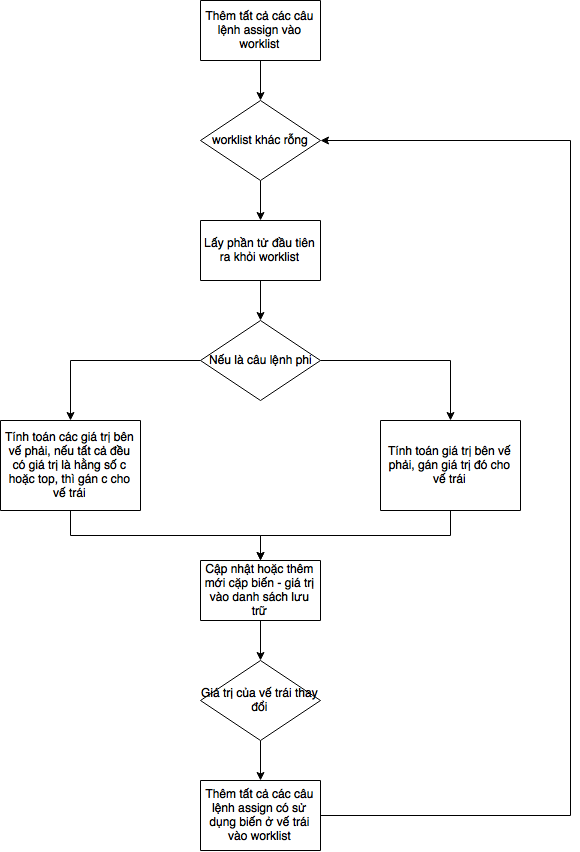
\includegraphics[scale=0.75]{image/constantPropagationAlgo}
	\caption{Giải thuật Constant propagation đã được điều chỉnh phù hợp với yêu cầu của trình dịch ngược}
	\label{fig:constantpropagationalgo}
\end{figure}

Để thể hiện giá trị của một biến có thể thuộc ba loại là \textit{top}, \textit{hằng số} hoặc \textit{bottom}, cần tạo ra một class mới để lưu trữ loại giá trị, đồng thời lưu trữ giá trị thực sự nếu biến đó là một hằng số. Class này được đặt tên là \textbf{ConstantVariable} và có khai báo được trình bày ở đoạn mã \ref{list:listconstexam5}
\begin{lstlisting}[caption={Đoạn mã thể hiện class ConstantVariable},label={list:listconstexam5}, language=c++]
class ConstantVariable{
	public:
	int type; //1: top, 2: constant, 3: bottom
	Exp* variable;
	ConstantVariable(){
		type = 3;
	}
};
\end{lstlisting}
Như vậy, mục tiêu của giải thuật này là tạo ra được một sơ đồ liên kết giữa một biến \textit{SSA} và một thực thể \textbf{ConstantVariable} thể hiện giá trị của biến đó. \\

Ngoài ra, để tính toán được giá trị thực sự của một biến, cần phải có một hàm chức năng nhận vào một biểu thức và trả về được giá trị của biểu thức đó. Có rất nhiều cách để hiện thực chức năng này, sau một quá trình xem xét, visitor sẽ được sử dụng cho việc tính toán giá trị của biểu thức. Visitor là một pattern design trong các chương trình lập trình hướng đối tượng, nó được dùng để tách một thuật toán ra khỏi cấu trúc dữ liệu mà thuật toán đó sử dụng. Lợi ích đạt được là người lập trình có thể thêm những chức năng mới cho cấu trúc dữ liệu đó mà không cần thay đổi kiến trúc của nó. Điều này phù hợp với nhu cầu hạn chế tối đa việc thay đổi các mã có sẵn khi hiện thực các giải pháp của luận văn trên một trình dịch ngược nào đó.\\

Để hiện thực pattern design này, cần tạo ra một class visitor và viết hàm visit cho các loại biểu thức. Các hàm visit này chính là nơi tính toán giá trị của biểu thức và trả về chúng. Vì biểu thức ở mức assembly thường được viết rất đơn giản, nên trong class visitor này chỉ cần có một số hàm visit cho các loại biểu thức sao đây:

\begin{itemize}
	\item \textit{Const}: Là biểu thức hằng số. Hàm visit này chỉ đơn giản trả về giá trị hằng số nếu đây là một hằng số nguyên.
	\item \textit{Binary}: Là biểu thức có 2 vế. Hàm visit sẽ visit từng vế của biểu thức, và nếu cả hai vế đều là hằng số, thì sẽ thực hiện phép tính cộng trừ nhân chia hai hằng số đó để ra được kết quả cuối cùng.
	\item \textit{RefExp}: Loại biểu thức này chứa một biểu thức khác, kèm theo câu lệnh khai báo biểu thức đó. Trong giới hạn nhu cầu của bài toán, chỉ những RefExp chứa biểu thức là một biến hoặc một thanh ghi được tính toán tiếp, còn những loại biểu thức kia sẽ mặc định trả về giá trị là bottom. Tên biến hoặc biểu thức sẽ được dò tìm trong bảng lưu trữ dữ liệu hằng số và bảng lưu trữ dữ liệu của câu lệnh \#DEFINE để tìm ra được giá trị thực sự của chúng và trả về.
	\item \textit{TypedExp}: Loại biểu thức để ép kiểu một biểu thức nào đó thành kiểu mong muốn. Với trường hợp này, giá trị trả về của biểu thức ép kiểu chính là giá trị của biểu thức con bên trong.
\end{itemize}


Như vậy, với phương pháp phân tích này, vấn đề vế phải của phép gán thanh ghi là những biểu thức phức tạp có hai toán hạng đã được giải quyết. Ngoài ra, phân tích này còn nhận biết được các biểu thức có giá trị giống nhau mặc dù hình thức bên ngoài khác nhau. Xem ví dụ các câu lệnh ở đoạn mã \ref{list:listdiffassignacc}. Câu lệnh gán số 1 và số 2 thực chất đều gán cho \textit{ACC} giá trị vùng nhớ có địa chỉ quy định bởi biến \textit{OPTIONS}. Nếu thực hiện phân tích Reaching definitions ở giải pháp trước, trình dịch ngược sẽ không thể biết được điều này. Tuy nhiên, ở giai đoạn này, vì trình dịch ngược sẽ tính toán được ở cả hai câu lệnh, \textit{ACC} đều mang giá trị của vùng nhớ có địa chỉ là \textbf{38}. Và ở những bước tiếp theo, trình dịch ngược sẽ đối chiếu giá trị \textbf{38} với bảng lưu trữ dữ liệu và biết được biến \textit{OPTIONS} đại diện cho giá trị đó.

\begin{lstlisting}[caption={Một số câu lệnh gán cho ACC có giá trị vế phải bằng nhau},label={list:listdiffassignacc}]
#DEFINE OPTIONS #38
#DEFINE CLAMP #37
...
MOV ACC, OPTIONS
MOV ACC, CLAMP+1
\end{lstlisting}

Phân tích Constant propagation sẽ trả về được giá trị thực sự của một biến, tuy nhiên, thanh ghi \textit{ACC} là một trường hợp đặc biệt. Khi gặp vế trái của câu lệnh khai báo là thanh ghi \textit{ACC}, giá trị thực sự không được quan tâm, mà chỉ giá trị của địa chỉ vùng nhớ đang được \textit{ACC} lưu giữ mới được xét đến. Như vậy, chỉ có các câu lệnh dạng \textbf{MOV ACC, [biểu thức]} sẽ được tính toán, còn khi gặp câu lệnh gán có dạng \textbf{MOV ACC, \#[biểu thức]} thì đoạn mã phân tích sẽ xem như giá trị của \textit{ACC} là \textit{bottom}. Như vậy, với các biến khác, giá trị lưu trong thực thể ConstantExpression tương ứng với biến đó là giá trị thực sự của biến, còn riêng với thanh ghi \textit{ACC}, giá trị đó được hiểu là giá trị địa chỉ vùng nhớ mà thanh ghi \textit{ACC} được load vào.
\section{Tìm kiếm mối quan hệ giữa các biến}
\subsection{Chuyển đổi giữa hằng số nguyên - biến byte tương ứng}
\label{sec:transfer}
Trước khi bước vào giai đoạn kiểm tra và ghi nhận mối quan hệ giữa các biến, trình dịch ngược cần phải giải quyết kết quả trả về của phương pháp phân tích Constant propagation ở trên. Như đã trình bày, phương pháp này cho biết chính xác giá trị địa chỉ vùng nhớ được lưu trữ bởi thanh ghi \textit{ACC}. Tuy nhiên, cần phải chuyển đổi con số này thành một biến byte có giá trị bằng nó vì mục đích cuối cùng của giải pháp vẫn là tìm mối quan hệ giữa các biến byte - biến bit. Có hai cách giải quyết vấn đề này:
\begin{itemize}
	\item Ở bất kỳ vị trí nào cần biết được biến byte đang quy định vùng nhớ lưu bởi ACC, lấy giá trị thực sự của địa chỉ vùng nhớ đó và dò tìm trong bảng lưu trữ dữ liệu các câu lệnh \#DEFINE để tìm ra biến byte tương ứng với giá trị đó.
	\item Tạm thời chấp nhận thay vì tìm kiếm mối quan hệ giữa biến byte - biến bit thì trình dịch ngược sẽ tìm kiếm mối quan hệ giữa giá trị trực tiếp - biến bit. Giá trị này chính là địa chỉ vùng nhớ mà thanh ghi ACC đang lưu trữ tại thời điểm sử dụng biết bit. Sau khi tìm ra các bộ giá trị - biến bit, thêm vào trình dịch ngược một bước chuyển đổi từ giá trị sang biến byte tương ứng dựa vào các câu lệnh khai báo giá trị biến byte ở chương trình đầu vào.
\end{itemize}

Hai giải pháp trên được mô tả lần lượt ở hình \ref{fig:waytotransfer1} và hình \ref{fig:waytotransfer2}. Qua hai sơ đồ trên, dễ dàng nhận ra giải pháp thứ hai sẽ giúp tiết kiệm thời gian xử lý chương trình hơn, nhờ vào việc chỉ cần truy xuất bảng dữ liệu ở cuối giai đoạn tìm kiếm. Còn giải pháp đầu tiên không hiệu quả do mỗi lần cần kiểm tra giá trị của thanh ghi \textit{ACC} lại phải tìm kiếm dữ liệu. Như vậy, giải pháp thứ hai sẽ được áp dụng.
\begin{figure} [h!]
	\centering
	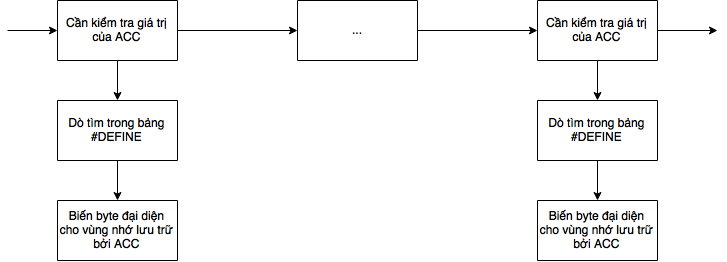
\includegraphics[width=0.7\linewidth]{image/wayToTransfer1}
	\caption{Giải pháp chuyển đổi giá trị - biến byte số 1}
	\label{fig:waytotransfer1}
\end{figure}
\begin{figure}[h!]
	\centering
	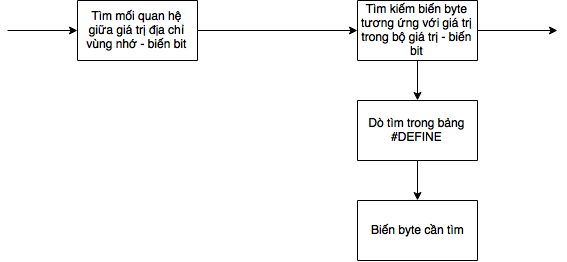
\includegraphics[width=0.7\linewidth]{image/wayToTransfer2}
	\caption{Giải pháp chuyển đổi giá trị - biến byte số 2}
	\label{fig:waytotransfer2}
\end{figure}
\subsection{Kiểm tra và ghi nhận mối quan hệ giữa các giá trị - biến bit}
 Nếu như ở giải pháp Kiểm tra kiểu, mối quan hệ biến byte - biến bit đã được cho trước và trình dịch ngược chỉ cần kiểm tra lại thì ở giải pháp này, vì không có thông tin từ phần chú thích của người lập trình, trình dịch ngược phải tự tìm kiếm các mối quan hệ đó, kiểm tra tính hợp lệ của chúng và ghi nhận vào danh sách dữ liệu. Các bước này được thể hiện ở hình \ref{fig:stepunionmaking}. Giai đoạn kiểm tra tính hợp lệ nhằm đảm bảo là các bộ biến được sử dụng theo đúng nguyên tắc đã giới thiệu ở chương đầu và cũng như ở giải pháp Kiểm tra kiểu trước đó, nếu có một câu lệnh nào đó vi phạm nguyên tắc sử dụng, trình dịch ngược sẽ báo lỗi và tiếp tục kiểm tra các câu lệnh tiếp theo để thuận tiện cho người dùng trong việc chỉnh sửa lỗi của chương trình assembly.
\begin{figure}[h]
	\centering
	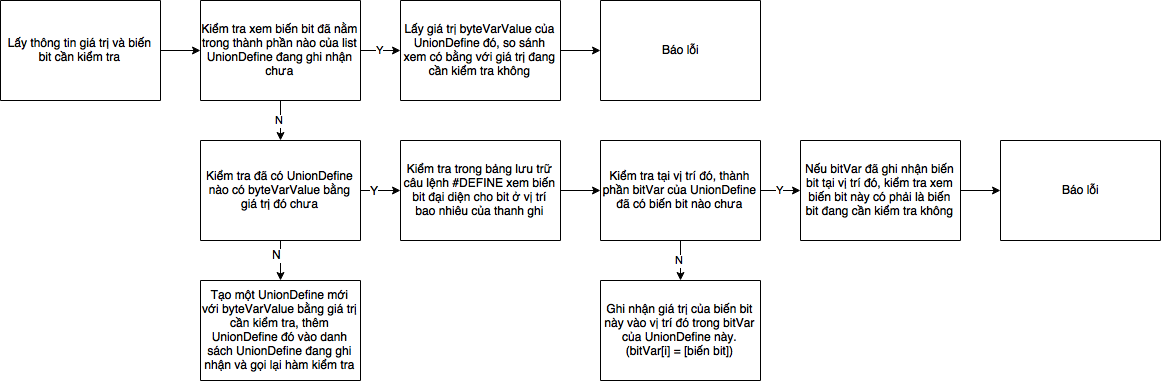
\includegraphics[width=0.7\linewidth]{image/stepUnionMaking}
	\caption{Các bước kiểm tra và ghi nhận dữ liệu vào danh sách UnionDefine}
	\label{fig:stepunionmaking}
\end{figure}

Như đã trình bày ở phần \ref{sec:transfer}, thay vì tìm kiếm các bộ biến byte - biến bit thì ở giai đoạn này sẽ tìm kiếm các bộ giá trị địa chỉ vùng nhớ - biến bit, vì vậy, cấu trúc lưu trữ dữ liệu tìm thấy được cũng phải được chỉnh sửa để ghi nhận mối quan hệ mới này. Cấu trúc UnionDefine được giới thiệu ở chương trước vẫn tiếp tục được sử dụng, tuy nhiên, được mở rộng thêm một trường dữ liệu mới là \textit{byteVarValue} để ghi nhận giá trị địa chỉ vùng nhớ của bộ biến. Đoạn mã mới được trình bày bên dưới.

\begin{lstlisting}[caption={Đoạn mã mới của class UnionDefine},label={list:listnewuniondefine},language=c++]
	class UnionDefine{
	public:
	char* byteVar;
	map<int, char*>* bitVar;
	int byteVarValue;
 };
\end{lstlisting}
Sau khi đã quét hết các câu lệnh trong chương trình và tìm được danh sách UnionDefine phù hợp, cần phải thêm vào một bước chuyển đổi từ giá trị thành biến byte đại diện cho giá trị đó. Điều này có thể được thực hiện bằng cách chạy vòng lặp qua bảng lưu trữ các câu lệnh \#DEFINE đã được thiết lập từ quá trình parse mã đầu vào. Nếu như có một giá trị nào đó chưa được khai báo ở câu lệnh \#DEFINE, một biến byte mới sẽ được sinh ra để đại diện cho giá trị ấy. Mẫu tên biến byte sẽ là LOCATION\_[giá trị của biến byte], ví dụ như LOCATION\_38.

Như vậy, giải pháp này đã giải quyết được các vấn đề đặt ra của luận văn. 